\label{ternary}

%бедно и непонятно, исправить обязательно. Может подумать о картинке в пример, дабы было нагляднее. 


В качеcтве операторов для данного алгоритма введем следующие несмещенные операторы: 
\begin{itemize}
   \item $flipOne(a)$ - изменение одного бита
   \item $flip'(a, b)$ - изменить один бит из совпадающего суффикса
   \item $xor3(a,b,c)$ - оператор исключающего ИЛИ для трех векторов 
\end{itemize}

(вставить формальное доказательство, что xor3 -> несмещенный)

Тогда рассмотрим следующий алгоритм: 
\begin{algorithm}[H]
\caption{Тернарный алгоритм}\label{lst1}
\begin{algorithmic}
        \State q_0 \leftarrow random
        \State s_1 \leftarrow $flipOne(q_0)$
		\While{true}
	        \State s_2 \leftarrow $flip'(q_0, s_1)$
            \State t_2 \leftarrow $xor3(q_0,s_1,s_2)$
            \State s_3 \leftarrow $flip'(q_0, t_2)$
            \State t_3 \leftarrow $xor3(q_0,s_2,s_3)$
            \State ...
		\EndWhile
\end{algorithmic}
\end{algorithm}

Таким образом формируется полное пространство поиска: 
\begin{example}
Пример генерации пространства для q_0 = [000...000]  \\
    q_0 = \{00000..0000\} \\
    s_1 = \{00000..0001\} \\
    s_2 = \{00000..0010\} \\
    t_2 = \{00000..0011\} \\
    s_3 = \{00000..0100\} \\
    t_3 = \{00000..0101\} \\
    ... \\
    t_k = \{10000..0000\} \\
    ... \\
\end{example}

%Размазано и непонятно. Переписать точно.
Таким образом пошагово генерируется все множество поиска без повторов. Сложность такого алгоритма равняется O($\frac{2^n + 1}{2}$), что равняется времени перебора всех векторов без повторов. Таким образом, верхняя и нижняя оценки сложности алгоритма совпадают. 


%Что-то вроде примера 
Рассмотрим класс некоторых задач, таких что экземпляром данной задачи является битовая строка из пространства поиска, размера $2^n$ от длины строки n. При этом у задачи существует единственный глобальный оптимум (при этом  наличие других оптимумов не важно). К таким задачам относится, например, OneMax.

\begin{figure}[H]
\caption{Дерево решений детерминированного алгоритма}\label{fig2}
    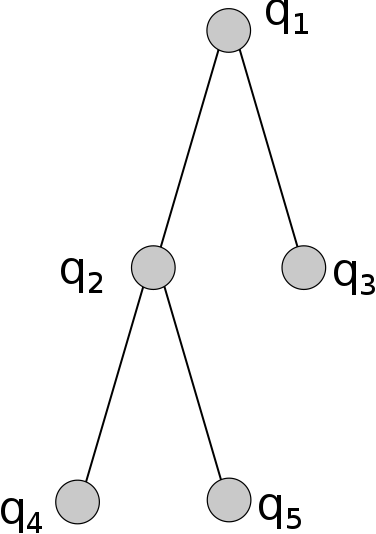
\includegraphics[height=5cm]{ITMO/pic/graph1.png}
\end{figure}


\begin{figure}[H]
\caption{Дерево решений другого оптимального алгоритма}\label{fig2}
    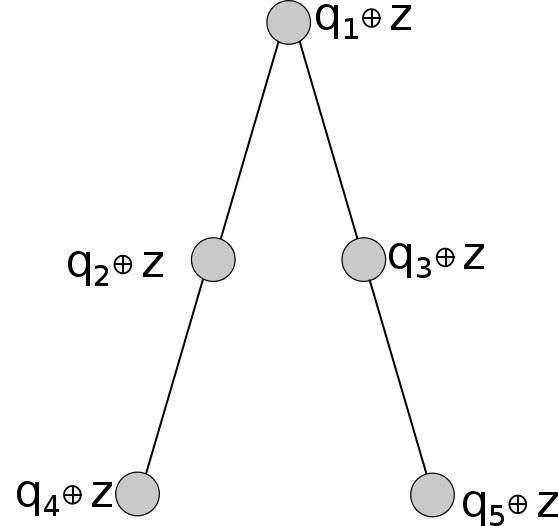
\includegraphics[height=10cm]{ITMO/pic/graph2.png}
\end{figure}

